%%%%%%%%%%%%%%%%%%%%%%%%%%%%%%%%%%%%%%%%%%%%%%%%%%%%%%%%%%%%%%%
%
% Welcome to Overleaf --- just edit your LaTeX on the left,
% and we'll compile it for you on the right. If you open the
% 'Share' menu, you can invite other users to edit at the same
% time. See www.overleaf.com/learn for more info. Enjoy!
%
%%%%%%%%%%%%%%%%%%%%%%%%%%%%%%%%%%%%%%%%%%%%%%%%%%%%%%%%%%%%%%%


% Inbuilt themes in beamer
\documentclass{beamer}
\newcommand{\mydet}[1]{\ensuremath{\begin{vmatrix}#1\end{vmatrix}}}
\usepackage[super]{nth}
\usepackage{amsmath}
% Theme choice:
\usetheme{CambridgeUS}

% Title page details: 
\title{Assignment 4}% \\ Indian Institute of Technology Hyderabad} 
\author{Malothu Avinash \\ AI21BTECH11018}
\date{\today}
% \logo{\large \LaTeX{}}


\begin{document}

% Title page frame
\begin{frame}
    \titlepage 
\end{frame}

% Remove logo from the next slides
% \logo{}


% Outline frame
\begin{frame}{Outline}
    \tableofcontents
\end{frame}


% Lists frame
\section{Question}
\begin{frame}{Question}
A fair die is rolled five times.We shall find p_5(2)\; that\;"six"\;will\;show\; twice
\end{frame}

\section{Answer}
\begin{frame}{Answer}
(a)In a single roll of die,
  
  A={six} is an event with probability 1/6 
  \\
  then
  \begin{align}
      &p=\frac{1}{6}\\
      &q=1-p\\
      &q=1-\frac{1}{6}\\
      &q=\frac{5}{6}\\
      &n=5;k=2\\
  \end{align}
\end{frame}
\begin{frame}
\begin{align}
     As\;p_n(k)&={}^{n}C_{k}\cdot (q)^{n-k} \cdot (p)^k\\
     p_5(2)&={}^{5}C_{2}\cdot (\frac{5}{6})^{3} \cdot (\frac{1}{6})^2
   \\&\text{Hence the probability of getting six twice in 5 rolls is}\\
     p_5(2)&=\frac{625}{3888}\\
     &=0.16075102880658423
\end{align}
\end{frame}
\begin{frame}{Code Output:}
The following is a result of python code plotting pmf of given cases
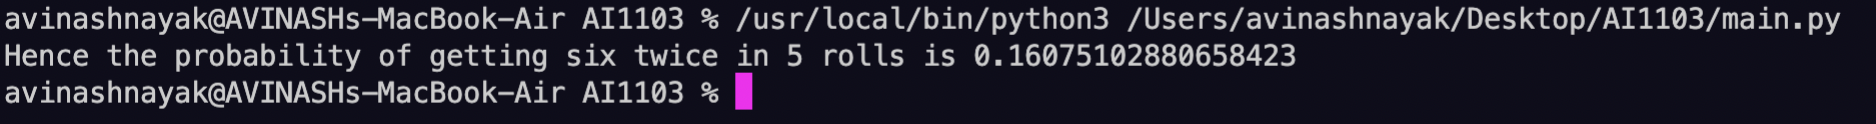
\includegraphics[width=\paperwidth]{solution.png}
\end{frame}

\end{document}
